\chapter{Separability Assumption on RIR Spectrogram}
\label{chapter:interspeech2018}

\section{NMF degradation models}
\begin{itemize}
\item Derivation
\begin{itemize}
\item NMF model for reverberation
\item Extended model for reverberation and noise
\end{itemize}
\end{itemize}
\section{Analysis of model}
\begin{itemize}
\item Effect of reverberation on clean speech bases and activation
\end{itemize}
\section{Enhancement algorithm}
\begin{itemize}
\item cost function
\item multiplicative update rule
\item normalization used 
\end{itemize}
\section{Experimental results}
\begin{itemize}
\item enhancement results
\item RIR estimates
\end{itemize}
\section{Discussion}
\begin{itemize}
\item comparison of results
\item limitations
\end{itemize}

\iffalse
In many real-world applications such as smart homes, robots, conference meetings, and voice-controlled personal assistants speech recordings are done using microphones placed few meters away from the source. Such distant speech recordings (DSRs) are severely affected by reverberation and background noise~\cite{naylor2010speech}. This degrades speech intelligibility and performance of automatic speech recognition performance (ASR) systems. Speech enhancement helps in improving speech intelligibility and can be used as a pre-processing step for improving ASR~\cite{kinoshita2016summary}. The effects of reverberation depend on the properties of speech and room impulse response (RIR). Speech dereverberation can be done using single- or multi-channel data depending on the application of interest. In this work, we address single-channel dereverberation in the DSR scenario.

Dereverberation methods proposed in the literature include reverberation cancellation methods, blind deconvolution based methods, and reverberation suppression methods such as spectral subtraction, linear prediction (LP) and non-negative matrix factorization (NMF) based methods~\cite{naylor2010speech}. The earliest work on NMF based dereverberation~\cite{kameoka2009robust} uses a convolutive NMF (referred as C-NMF) model for the reverb spectrogram. Since then many modifications to this have been proposed both in single-channel~\cite{Kumar2011,mohammadiha2016speech,Mohammadiha2015,baby2015coupled,Kallasjoki2014} and multi-channel scenario~\cite{Mirsamadi2014}. In~\cite{Kallasjoki2014}  the C-NMF model is shown as a special case of NMF decomposition. The C-NMF model for speech dereverberation was improved by additionally incorporating a NMF model for clean speech~\cite{mohammadiha2016speech, Mohammadiha2015}. Various supervised approaches to handle reverberation in noisy environments have also been proposed~\cite{baby2015coupled, baby2016phd, baby2017joint}.  
Different regularization on RIRs in single-channel~\cite{baby2017joint,mohanan2017speech} and multi-channel~\cite{Yu2014} scenario have been proposed leading to better speech enhancement. In contrast to these methods that use C-NMF for dereverberation, we propose a NMF model for reverberation. The model uses magnitude spectrogram of the reverb speech and learned clean speech bases to estimate the enhanced speech. Such an approach will allow us to incorporate meaningful constraints in the frequency- and time-domain. This leads to a better speech enhancement, as it has direct control over the estimates of clean speech activations and better RIR estimates. Another advantage of such a model is that it can be easily extended to handle additive noise making it suitable for a noisy reverberant scenario. 
%The NMF methods are evaluated using speech enhancement measures such as CD and SRMR~\cite{hu2008evaluation, falk2010non}.
%Dereverberation methods proposed in the literature include reverberation cancellation methods, blind deconvolution based methods and reverberation suppression methods such as spectral subtraction, linear prediction (LP) based methods~\cite{naylor2010speech}. We propose a reverberation suppression method based on non-negative matrix factorization (NMF). The model uses magnitude spectrogram of the reverb speech and clean speech bases to estimate the enhanced speech.
%The earliest work on NMF based dereverberation~\cite{kameoka2009robust} uses a convolutive NMF (referred as C-NMF) model for the reverb spectrogram. Since then many  modifications to this have been proposed both in single-channel~\cite{Kumar2011,mohammadiha2016speech,Mohammadiha2015,baby2015coupled,Kallasjoki2014} and multi-channel scenario~\cite{Mirsamadi2014}. The original C-NMF model for speech dereverberation was improved by incorporating NMF models for the speech signals~\cite{mohammadiha2016speech, Mohammadiha2015}. Various supervised approaches to handle reverberation and noise have been proposed to handle reverberation in noisy environments~\cite{baby2015coupled, baby2016phd, baby2017joint}. In~\cite{Kallasjoki2014}  the C-NMF model is viewed as a NMF decomposition.
%Different regularization on RIRs in single-channel~\cite{baby2017joint,mohanan2017speech} and multi-channel~\cite{Yu2014} scenario have been proposed leading to better speech enhancement. In contrast to these methods that use C-NMF for dereverberation, we propose a NMF model for reverberation. Such an approach will allow us to incorporate meaningful constraints in the frequency- and time-domain. This leads to a better speech enhancement, as it has direct control over the estimates of clean speech activations and better RIR estimates. Another advantage of such a model is that it can be easily extended to handle additive noise making it suitable for noisy reverberant scenario. The NMF methods are evaluated using speech enhancement measures such as CD and SRMR~\cite{hu2008evaluation, falk2010non}.


\section{NMF based dereverberation}

Reverberated speech $y(t)$ recorded at a microphone is expressed as the convolution of clean speech $s(t)$ and the RIR $h(t)$~\cite{naylor2010speech}. %\textbf{[($y(t)=s(t)*h(t)$)]}~\cite{naylor2010speech}.
%\begin{equation}
%y(t) = h(t) * s(t)
%\label{eq:deg1}
%\end{equation}
%In the magnitude spectrogram domain, the degradation is approximated as the sum of spectrograms due to reverberation and noise. 
%\subsection{C-NMF model for reverberation}
In the absence of noise, speech degradation due to reverberation can be modeled in the magnitude spectrogram domain by utilizing the modulation transfer function (MTF) model for reverberation~\cite{kameoka2009robust}. According to the MTF  model, the magnitude envelope for each subband of reverberant speech magnitude spectrogram ($\mathbf{Y}$) can be approximated as the convolution of the corresponding subband magnitude envelopes of the RIR ($\mathbf{H}$) and the clean speech ($\mathbf{S}$) spectrograms~\cite{Kumar2011}. Accordingly, 
\begin{equation}
Y(k,n) \approx H(k,n)*_n S(k,n)=\sum_{l=0}^{L_h-1}H(k,l)S(k,n-l)\text{,}
\label{eq:deg2}
\end{equation}
where, $Y(k,n)$, $H(k,n)$ and $S(k,n)$ represent the $(n,k)$-th element of $\mathbf{Y}$, $\mathbf{H}$ and $\mathbf{S}$, respectively, $L_h$ represents the number of frames used to represent the RIR spectrogram $\mathbf{H}$ and $*_n$ represents convolution across frame index. The model in~(\ref{eq:deg2}) can be viewed as a convolutive NMF (C-NMF) decomposition where $\mathbf{H}$ and $\mathbf{S}$ can be obtained using multiplicative updates~\cite{kameoka2009robust}.

%The model in (\ref{eq:deg2}) was improved in \cite{mohammadiha2016speech,Mohammadiha2015} to use a NMF model for speech spectrogram. 
The speech enhancement results using the model in (\ref{eq:deg2}) were improved by incorporating a NMF model for the magnitude spectrogram of clean speech~\cite{mohammadiha2016speech,Mohammadiha2015}.
They exploit the low-rank nature of clean speech spectrogram by having a NMF decomposition on clean speech spectrogram $S(k,n)$ as,
\begin{equation}
S(k,n)\approx\sum_{r=1}^R W_{s}(k,r)X_{s}(r,n)\text{,}
\label{eq:nmf1}
\end{equation}
where $W_{s}(k,r)$, $X_s(r,n)$ are elements of the bases, activations and $R$ is the rank of the decomposition. Using (\ref{eq:nmf1}) in (\ref{eq:deg2}),
\begin{equation}
Y(k,n) \approx \sum_{l=0}^{L_h-1}H(k,l)\bigg(\sum_{r=1}^R W_{s}(k,r)X_{s}(r,n-l)\bigg)\text{.}
\label{eq:deg4}
\end{equation}
From (\ref{eq:deg4}), enhanced speech is obtained by solving for $H(k,l)$, $W_{s}(k,r)$ and $X_{s}(r,n)$ iteratively. This method will be referred to as C-NMF+NMF. In \cite{mohammadiha2016speech,Mohammadiha2015}, several approaches to obtain bases are experimented with. In online (unsupervised) methods, the bases are learned from the reverberant speech. In offline (supervised) methods, the bases are learned from clean speech utterances. The proposed approach uses supervised bases, so we use the offline method as a baseline for comparison. The joint speech dereverberation and denoising methods using C-NMF model~\cite{baby2015coupled, baby2016phd, baby2017joint} are not compared as they use exemplar bases, which require a large number of bases when compared to learned bases to represent clean speech.   

%\subsection{Proposed non-convolutive NMF model for reverberation}
\subsection{Proposed non-convolutive NMF model}
\label{sec:PropNMF}
%In the proposed method, an alternate approach to perform dereverberation using NMF is discussed. A two stage algorithm is proposed to perform dereverberation. In the first stage, a supervised NMF decomposition is performed on reverb spectrogram. This stage assumes that the clean speech basis can model reverb spectogram. The basis vectors are learned from clean utterances. In the second stage, clean speech activations are obtain from the reverb activations using a CNMF decomposition. The two stage approach is made possible by having additional constrain on RIR spectrogram that it varies similarly in different subbands ($H(f,n)=H(n)\forall f$). Mathematically, the two stages can be written as,
We propose a method to perform dereverberation by representing the reverb spectrogram using a non-convolutive NMF as, $\mathbf{\tilde{Y}}=\mathbf{W}_R\mathbf{X}_R$, where $\mathbf{W}_R$ and $\mathbf{X}_R$ represent the bases and activation of this decomposition. Such a model is made possible by having a separability assumption on the RIR spectrogram $H(n,k)=H_1(k)H_2(n)$. 
This approximation is based on the following observations. 
Firstly, the RIR magnitude spectrum across frequencies for different frames is similar and has a decaying structure across time as is observed in literature~\cite{wen2008blind}. Secondly, the subband magnitudes of the RIR for different frequencies decay with time. The rate of decay with time for different subband is assumed to be same. Combining these observations, a simplifying model will be to write $H(n,k)$ as having a frequency envelope $H_1(k)$ with a gain $H_2(n)$ for different frames.
%The algorithm can be improved by incorporating the frequency dependence of $T_{60}$~\cite{jeub2010we}.
%Firstly, the RIR spectrogram for different frames approximately follows the same frequency structure. It can be observed that some frequency bands of RIR spectrogram have higher magnitude while others have lower values. The presence of frequency envelope for RIR spectrogram is also reported in the literature~\cite{wen2008blind}.  Secondly, the magnitudes of RIR spectrograms for all frequency bands decay down with time.  Combining these observations, a simplifying model will be to write $H(n,k)$ as having a frequency envelope $H_1(k)$ with a gain $H_2(n)$ for different frames. The frequency dependence of $T_{60}$~\cite{jeub2010we} is ignored in this assumption.}
With this, we have
%This model is based on MTF model for reverberation. With a separability assumption on RIR spectrogram ($H(n,k)=H_1(k)H_2(n)$), the MTF model is replaced with a NMF model. $\mathbf{W}_R$ and $\mathbf{X}_R$ represents the bases and activation of this decomposition. The reverb spectrogram ($\tilde{\mathbf{Y}}$) can be is written as,

\begin{align}
\tilde{Y}&(k,n) = \sum_{l=0}^{L_h-1} H_1(k)H_2(l) \sum_{r=1}^R W_{s}(k,r)X_{s}(r,n-l)\nonumber\\
& = \sum_{r=1}^R \underbrace{W_s(k,r)H_1(k)}_{W_R(k,r)} \underbrace{\sum_{l=0}^{L_h-1}H_2(n)X_s(r,n-l)}_{X_R(r,n)}
\label{eq:reverbNMF}
\end{align}
where, $\tilde{Y}(i,j)$, $W_R(i,j)$, and $X_R(i,j)$ are the $(i,j)$-th element of $\tilde{\mathbf{Y}}$, $\mathbf{W}_R$ and $\mathbf{X}_R$, respectively. Equation~(\ref{eq:reverbNMF}) is a NMF decomposition with rank $R$ of the reverb spectrogram. The set of bases and activations obtained from this decomposition is related to clean speech bases and activations. The reverb bases ($W_R(k,r)=W_s(k,r)H_1(k)$) are the clean speech bases $W_s(k,r)$ modified by the frequency envelope of the RIR spectrogram $H_1(k)$.
%All the clean speech bases are modified by a frequency envelope RIR spectrogram ($H_1(k)$) to obtain the reverb bases ($W_R(k,r)=W_s(k,r)H_1(k)$). 
The reverb activations are obtained as the convolution of clean speech activations with the time-dependent envelope of the RIR ($X_R(r,n)=X_s(r,n)*_nH_2(n)$). Estimation of these parameters is done in two steps. In the first step, with the knowledge of learned speech bases, $H_1(k)$ and reverb activations are learned from the reverb spectrogram. Generalized Kullback-Leibler (KL) divergence is used as the distance measure in the first stage as this is related to speech~\cite{mohammadiha2016speech}. The NMF cost function ($C$) is given as, 
\begin{equation}
C = \sum_{n,k} \bigg[Y(k,n)\text{ln}\bigg(\dfrac{Y(k,n)}{\tilde{Y}(k,n)}\bigg) - Y(k,n) + \tilde{Y}(k,n)\bigg]
\label{eq:C}
\end{equation}
Multiplicative update rules are obtained for $H_1(k)$ and $X_R(r,n)$ using the cost function in (\ref{eq:C}). The updates obtained are,
\begin{align}
H_1(k)&\leftarrow H_1(k) \dfrac{\sum_{n,r} \dfrac{Y(k,n)}{\tilde{Y}(k,n)} W_s(k,r)X_R(r,n)}{\sum_{n,r} W_s(k,r)X_R(r,n)}\text{, and}\nonumber\\
X_R(r,n)&\leftarrow X_R(r,n) \dfrac{\sum_k \dfrac{Y(k,n)}{\tilde{Y}(k,n)}H_1(k)W_s(k,r)}{\sum_k H_1(k)W_s(k,r)}
\label{eq:updateProp}
\end{align} 
In the second stage, clean activations are learned from reverb activations. The second stage uses Euclidean distance as the distance measure to estimate clean activations from reverb activations, since the estimated parameters are no longer related to speech as in (\ref{eq:C}) and can be viewed as a general signal. The NMF cost function in this case is defined as,
\begin{equation}
C_1 = \sum_{r,n}( X_R(r,n) - H_2(n) *_n X_s(r,n))^2
\end{equation}
Simultaneous estimation of $X_s(r,n)$ and $H_2(n)$ from $X_R(r,n)$ leads to the trivial solution of $X_s(r,n)=X_R(r,n)$ and $H_2(n)$ being an impulse. To get a meaningful solution, $H_2(n)$ is initialized using prior knowledge of room and source-microphone distance in the RIR structure (Sec 4.1.3 in~\cite{kinoshita2016summary}).
% and $X_s(r,n)$ is updated. For example, Sec 4.1.3 in~\cite{kinoshita2016summary} discusses a model for time-dependent behavior of $H(n,k)$ using the knowledge of $T_{60}$. 
The update for $X_s(r,n)$ is given by,
\begin{equation}
X_s(r,p) \leftarrow X_s(r,p) \dfrac{\sum_n X_R(r,n)H_2(n-p)}{\sum_n\tilde{X}_R(r,n) H_2(n-p)}
\end{equation}
where, $\tilde{X}_R(r,n)$ is the estimated reverb activation ($\tilde{X}_R(r,n) = X_s(r,n)*_nH_2(n)$). The clean speech spectrogram can be estimated as $\hat{S}(k,n)=G(k,n)Y(k,n)$, where the gain function $G(k,n)$ is written as,
\begin{equation}
G(k,n)=\dfrac{\sum_rW_s(k,r)X_s(r,n)}{\tilde{Y}(n,k)}
\end{equation}
The proposed reverberation model using NMF will be referred to as R-NMF. 

We now justify the proposed model using an illustrative example, considering a reverberated TIMIT utterance obtained using a RIR with $T_{60}\approx700$~ms and source-microphone distance (d) of $0.5$~m. Using the first step, one can see that the reverb bases $W_R(k,r)$ are indeed the clean speech bases $W_s(k,r)$ acted upon by the frequency envelope of the RIR $H_1(k)$. The estimated frequency envelope of the RIR obtained using the proposed model is compared with the true frequency envelope $H^{\text{True}}_1(k)$ in Figure~\ref{fig:freqEnv_comp}. $H^{\text{True}}_1(k)$ is obtained as the average value of normalized frequency spectrum for the three frames of RIR spectrogram with maximum energy. From the figure, it is clear that for most frequencies, the estimated $H_1(k)$ is very close to $H^{\text{True}}_1(k)$. A similar behavior was observed for other RIRs. 

\begin{figure}[tbh!]
  \centering
  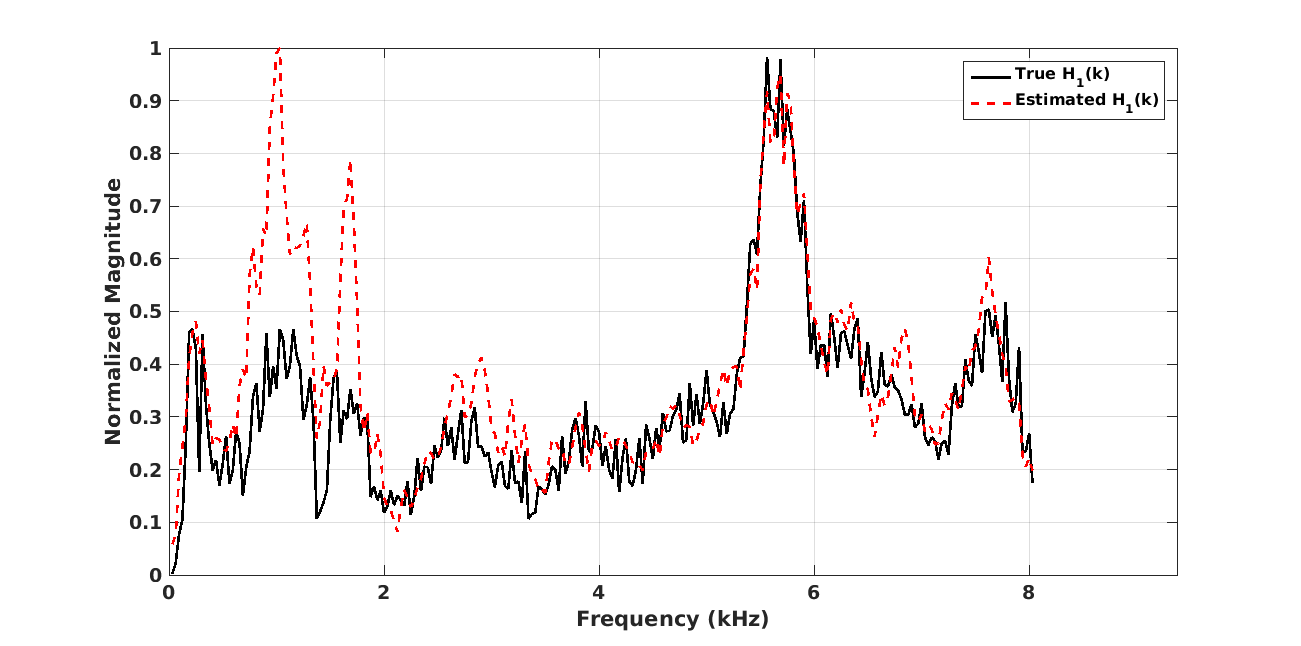
\includegraphics[width=8.2cm, height=4.5cm]{fig/freqEnv_comparison.png}
  \caption{Comparison of the estimated frequency envelope $H_1(k)$ to that of the true frequency envelope $H^{True}_1(k)$ for a measured RIR with $T_{60}\approx 700$~ms and $d=0.5$~m.}
  \label{fig:freqEnv_comp}
\end{figure}

The second step of the proposed approach can be justified by showing that the clean speech activations can be obtained from a deconvolution of the reverb activations and $H_2(k)$. Figure~\ref{fig:activation_comp} compares the activations obtained using the different NMF models for a specific basis, which is obtained from the NMF decomposition of the reverberated utterance. The clean speech activations (shown in Figure~\ref{fig:activation_comp}(a)) spread due to the effect of reverberation as is shown in Figure~\ref{fig:activation_comp}(b). Dereverberation using the proposed approach helps in reducing this effect. This is evident from the activations estimated using the R-NMF method as shown in Figure~\ref{fig:activation_comp}(d). The C-NMF+NMF method (shown in Figure~\ref{fig:activation_comp}(c)) was unable to completely recover the clean activations in this case. In our experiments, it was observed that the R-NMF consistently obtained the clean activations, whereas the C-NMF+NMF was not consistent. 
\begin{figure}[tbh!]
  \centering
  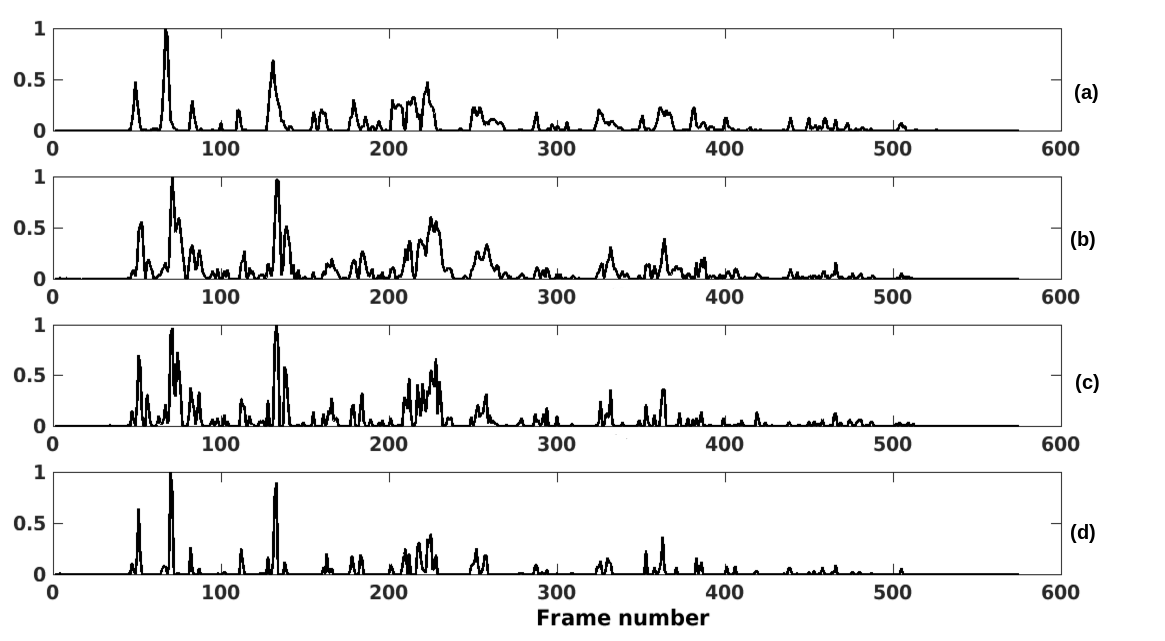
\includegraphics[width=8.5cm, height=6cm]{fig/activation_comparison4.png}
  \caption{Normalized activations obtained for a test utterance. (a) Clean utterance, (b) Reverb utterance, (c) Dereverberation using C-NMF+NMF, (d) Dereverberation using R-NMF. The estimated activations in (d) are similar to   
the true activations in (a).}
  \label{fig:activation_comp}
\end{figure}
The overall enhancement obtained using the R-NMF and C-NMF+NMF is in Figure~\ref{fig:speech_production} by comparing the enhanced spectrograms with the clean and reverb spectrograms. It can be seen that the R-NMF was more effective in removing the artifacts caused due to reverberation. This is clearly visible in the silence regions as indicated by the red boxes.
%Due to reverberations, speech spectrum spreads into the silence region. The method is able to reduce this effect.
\begin{figure}[tbh!]
  \centering
  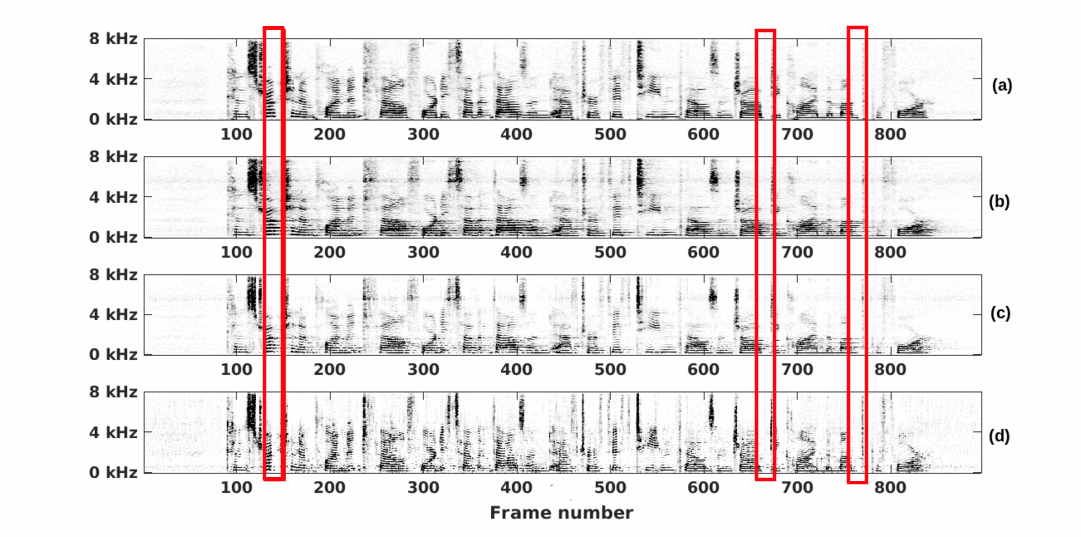
\includegraphics[width=8.5cm, height=5cm]{fig/spectrogram_prop3.png}
  \caption{Spectrogram of (a) Clean speech, (b) Reverb speech, (c) Enhanced speech using C-NMF+NMF, and (d) Enhanced speech using the proposed R-NMF. The regions where R-NMF performs better is shown using red boxes.}
  \label{fig:speech_production}
\end{figure}

%\subsection{Non-convolutive NMF model for reverberation and noise}
\subsection{Proposed model for reverberation and noise}
One of the advantages of having the NMF model for reverberation as proposed in (\ref{eq:reverbNMF}) is that it can be easily extended to include a NMF model for additive noise. The time-domain degraded speech can be represented as $y_D(t)=y(t)+z(t)$. The corresponding magnitude spectrogram $\mathbf{Y}_D$ can be approximated as the sum of reverberation spectrogram $\tilde{\mathbf{Y}}$ and noise spectrogram $\mathbf{Z}$~\cite{baby2015coupled,baby2016phd,baby2016supervised}. Further, the noise spectrogram can also be decomposed using a NMF model ($\mathbf{Z}=\mathbf{W}_n\mathbf{X}_n$)~\cite{wilson2008speech}. Hence,
\begin{align}
\tilde{Y}_D(k,n) &= \tilde{Y}(k,n)+Z(k,n) \text{,}\label{eq:NMFdeg}\\
\text{where }Z(k,r)&=\sum_{r=1}^{R_n} W_{n}(k,r)X_{n}(r,n)\text{.}
\end{align}
$\tilde{Y}_D(k,n)$, $Z(k,n)$ represent the $(k,n)$-th element of ${\tilde{\mathbf{Y}}_D}$, $\mathbf{Z}$, respectively, with $W_{n}(k,r)$ and $X_{n}(r,n)$ representing the bases and activations for the noise spectrogram and $R_n$ the rank of NMF decomposition for $\mathbf{Z}$. The model in (\ref{eq:NMFdeg}) can be written as,
\begin{align}
\tilde{\mathbf{Y}}_D = \mathbf{W}_R\mathbf{X}_R + \mathbf{W}_n\mathbf{X}_n = [\mathbf{W}_R | \mathbf{W}_n] [\mathbf{X}_R^T | \mathbf{X}_n^T]^T
\label{eq:degNMF}
\end{align}
%\begin{align}
%\tilde{\mathbf{Y}}_D &= \mathbf{W}_R\mathbf{X}_R + \mathbf{W}_n\mathbf{X}_n\nonumber \\
%& = [\mathbf{W}_R | \mathbf{W}_n] [\mathbf{X}_R^T | \mathbf{X}_n^T]^T
%\label{eq:degNMF}
%\end{align}
The bases for the decomposition are the combined bases of reverb and noise spectrograms. The reverb basis $W_R(k,r)$ depends on clean speech basis $W_s(k,r)$ as $W_R(k,r)=W_s(k,r)H_1(k)$. Activations for the decomposition in (\ref{eq:degNMF}) are the combined activations of reverberation and noise activations. The parameters $H_1(k)$, $\mathbf{X}_R$ and $\mathbf{X}_n$ are estimated using multiplicative update rules for the cost function, similar to~(\ref{eq:C}), except that $Y(n,k)$ and $\tilde{Y}(n,k)$ is replaced by $Y_D(n,k)$ and $\tilde{Y}_D(n,k)$.
%\begin{equation}
%C_D = \sum_{n,k} \bigg[Y_D(k,n)\text{ln}\bigg(\dfrac{Y_D(k,n)}{\tilde{Y}_D(k,n)}\bigg) - Y_D(k,n) + \tilde{Y}_D(k,n)\bigg]
%\end{equation}
The update rules for $H_1(k)$ and $\mathbf{X}_R$ are similar to the updates in equation (\ref{eq:updateProp}), except that $Y(k,n)$ and $\tilde{Y}(k,n)$ are replaced by $Y_D(k,n)$ and $\tilde{Y}_D(k,n)$, respectively. Update of $\mathbf{X}_n$ is obtained as,
\begin{equation}
X_n(n,r) \leftarrow X_n(n,r) \dfrac{\sum_k \dfrac{Y_D(k,n)}{\tilde{Y}_D(k,n)}W_n(k,r)}{\sum_k W_n(k,r)}
\end{equation}
We will refer to this model as R-NMF+NMF.
%Here an NMF model is assumed for the noise spectrogram.  The enhanced speech is estimated by simultaneously solving for $H(f,n)$, $X_s(r,n)$ and $X_n(r,n)$. The objective function to be minimized is a non-convex function and is liable to give unsatisfactory solution. Sparsity constrain are added to the clean and noise activations to improve the performance.

%\begin{table*}[htb]
%\centering
%\caption{Relative improvements in objective measures for the reverberant data at $20$~dB SNR.}
%\label{tab:20dB}
%\begin{tabular}{|l|l|l|l|l|l|l|l|l|l|l|l|l|ll}
%\cline{1-13}
%\multirow{2}{*}{} & \multicolumn{4}{c|}{CD}                                       & \multicolumn{4}{c|}{SRMR}                                     & \multicolumn{4}{c|}{PESQ}                                     &  &  \\ \cline{2-13}
%                  & RIR1          & RIR2          & RIR3          & RIR4          & RIR1          & RIR2          & RIR3          & RIR4          & RIR1          & RIR2          & RIR3          & RIR4          &  &  \\ \cline{1-13}
%Degraded speech   & 3.92          & 4.78          & 4.06          & 4.82          & 4.89          & 2.59          & 3.98          & 2.37          & 2.52          & 1.93          & 2.41          & 1.92          &  &  \\ \cline{1-13}
%C-NMF+NMF         & 4.27          & 4.50          & 4.39          & 4.60          & \textbf{5.71} & \textbf{4.33} & \textbf{5.62} & 4.51          & \textbf{2.74} & \textbf{2.33} & \textbf{2.69} & \textbf{2.33} &  &  \\ \cline{1-13}
%R-NMF             & \textbf{3.73} & \textbf{4.35} & 3.89          & \textbf{4.23} & 5.52          & 3.93          & 4.90          & 4.24          & 2.71          & 2.12          & 2.56          & 2.12          &  &  \\ \cline{1-13}
%R-NMF+NMF         & 3.76          & 4.53          & \textbf{3.83} & 4.47          & \textbf{5.71} & 4.14          & 5.32          & \textbf{4.26} & 2.67          & 2.00          & 2.52          & 2.00          &  &  \\ \cline{1-13}
%\end{tabular}
%\end{table*}
\begin{table*}[htb]
\centering
\caption{Comparison of objective measures for the reverberant and noisy speech, with stationary noise at $10$~dB SNR}
\label{tab:10dB}
\begin{tabular}{|l|l|l|l|l|l|l|l|l|}
\hline
\multirow{2}{*}{} & \multicolumn{4}{c|}{CD}                                       & \multicolumn{4}{c|}{SRMR}                                     \\ \cline{2-9} 
                  & RIR1          & RIR2          & RIR3          & RIR4          & RIR1          & RIR2          & RIR3          & RIR4          \\ \hline
Degraded speech   & 4.98          & 5.43          & 5.07          & 5.46          & 3.24          & 2.08          & 3.03          & 1.92          \\ \hline
C-NMF+NMF~\cite{mohammadiha2016speech,Mohammadiha2015}         & 5.28          & 5.35          & 5.38          & 5.45          & 4.69          & 3.71          & 4.70          & 3.85          \\ \hline
R-NMF             & 4.85          & 5.16          & 4.97          & 5.26          & 4.16          & 3.43          & 3.99          & 3.73          \\ \hline
R-NMF+NMF          & \textbf{4.40} & \textbf{4.49} & \textbf{4.49} & \textbf{4.48} & \textbf{5.37} & \textbf{4.08} & \textbf{5.20} & \textbf{4.12} \\ \hline
\end{tabular}
\end{table*}
%\begin{table*}[htb]
%\centering
%\caption{Relative improvements in objective measures for the reverberant data at $10$~dB SNR.}
%\label{tab:10dB}
%\begin{tabular}{|l|l|l|l|l|l|l|l|l|l|l|l|l|ll}
%\cline{1-13}
%\multirow{2}{*}{} & \multicolumn{4}{c|}{CD}                                       & \multicolumn{4}{c|}{SRMR}                                     & \multicolumn{4}{c|}{PESQ}                                     &  &  \\ \cline{2-13}
%                  & RIR1          & RIR2          & RIR3          & RIR4          & RIR1          & RIR2          & RIR3          & RIR4          & RIR1          & RIR2          & RIR3          & RIR4          &  &  \\ \cline{1-13}
%Degraded speech   & 4.98          & 5.43          & 5.07          & 5.46          & 3.24          & 2.08          & 3.03          & 1.92          & 2.09          & 1.73          & 2.06          & 1.73          &  &  \\ \cline{1-13}
%C-NMF+NMF         & 5.28          & 5.35          & 5.38          & 5.45          & 4.69          & 3.71          & 4.70          & 3.85          & 2.24          & \textbf{2.01} & \textbf{2.24} & \textbf{2.06} &  &  \\ \cline{1-13}
%R-NMF             & 4.85          & 5.16          & 4.97          & 5.26          & 4.16          & 3.43          & 3.99          & 3.73          & 2.15          & 1.85          & 2.08          & 1.86          &  &  \\ \cline{1-13}
%R-NMF+NMF         & \textbf{4.40} & \textbf{4.49} & \textbf{4.49} & \textbf{4.48} & \textbf{5.37} & \textbf{4.08} & \textbf{5.20} & \textbf{4.12} & \textbf{2.31} & 1.81          & 2.20          & 1.89          &  &  \\ \cline{1-13}
%\end{tabular}
%\end{table*}
\begin{table*}[hbt]
\centering
\caption{Comparison of objective measures for the reverberant and noisy speech, with non-stationary noise (Factory) at $10$~dB SNR}
\label{tab:10dBnonStat}
\begin{tabular}{|l|l|l|l|l|l|l|l|l|}
\hline
\multirow{2}{*}{} & \multicolumn{4}{c|}{CD}                                       & \multicolumn{4}{c|}{SRMR}                                     \\ \cline{2-9} 
                  & RIR1          & RIR2          & RIR3          & RIR4          & RIR1          & RIR2          & RIR3          & RIR4          \\ \hline
Degraded speech   & 5.28          & 5.63          & 5.36          & 5.68          & 3.53          & 2.22          & 3.25          & 2.05          \\ \hline
C-NMF+NMF~\cite{mohammadiha2016speech,Mohammadiha2015}         & 5.60          & 5.65          & 5.75          & 5.82          & 4.81          & 3.83          & 4.83          & 3.99          \\ \hline
R-NMF             & 5.16          & 5.43          & 5.28          & 5.55          & 4.50          & 3.53          & 4.30          & 3.84          \\ \hline
R-NMF+NMF          & \textbf{4.77} & \textbf{5.12} & \textbf{4.80} & \textbf{5.17} & \textbf{5.50} & \textbf{4.32} & \textbf{5.15} & \textbf{4.31} \\ \hline
\end{tabular}
\end{table*}
%\begin{table*}[hbt]
%\centering
%\caption{Relative improvements in objective measures for the reverberant data for non-stationary noise (Factory) added at $10$~dB SNR.}
%\label{tab:10dBnonStat}
%\begin{tabular}{|l|l|l|l|l|l|l|l|l|l|l|l|l|ll}
%\cline{1-13}
%\multirow{2}{*}{} & \multicolumn{4}{c|}{CD}                                       & \multicolumn{4}{c|}{SRMR}                                     & \multicolumn{4}{c|}{PESQ}                                     &  &  \\ \cline{2-13}
%                  & RIR1          & RIR2          & RIR3          & RIR4          & RIR1          & RIR2          & RIR3          & RIR4          & RIR1          & RIR2          & RIR3          & RIR4          &  &  \\ \cline{1-13}
%Degraded speech   & 5.28          & 5.63          & 5.36          & 5.68          & 3.53          & 2.22          & 3.25          & 2.05          & 2.15          & 1.74          & 2.10          & 1.75          &  &  \\ \cline{1-13}
%C-NMF+NMF         & 5.60          & 5.65          & 5.75          & 5.82          & 4.81          & 3.83          & 4.83          & 3.99          & \textbf{2.28} & \textbf{2.03} & \textbf{2.26} & \textbf{2.05} &  &  \\ \cline{1-13}
%R-NMF             & 5.16          & 5.43          & 5.28          & 5.55          & 4.50          & 3.53          & 4.30          & 3.84          & 2.22          & 1.86          & 2.13          & 1.88          &  &  \\ \cline{1-13}
%R-NMF+NMF         & \textbf{4.77} & \textbf{5.12} & \textbf{4.80} & \textbf{5.17} & \textbf{5.50} & \textbf{4.32} & \textbf{5.15} & \textbf{4.31} & 2.25          & 1.76          & 2.19          & 1.74          &  &  \\ \cline{1-13}
%\end{tabular}
%\end{table*}
\section{Results}
The performance of the algorithms in Sec. 2 was compared using speech enhancement measures. As mentioned earlier, we do not consider~\cite{baby2015coupled, baby2016phd, baby2017joint} as these are exemplar based methods.

\subsection{Dataset and experiments}
%The speech enhancement performance was compared using the TIMIT database \cite{garofolo1993timit}.
The speech enhancement performance was assessed using a subset of $16$ speakers, with ten utterances per speaker from the TIMIT database~\cite{garofolo1993timit}. One utterance spoken by each speaker was used for testing.
%A subset of $16$ different sentences spoken by $16$ distinct speakers was used for testing. 
For the NMF representation, $100$ speaker specific clean speech bases were learned from $9$ utterances different from the one used in testing of that speaker.
Four measured RIRs from the REVERB challenge \cite{kinoshita2016summary} were used for the evaluation. The RIRs correspond to two different rooms and two different source-microphone distances : near ($0.5$~m) and far ($2$~m) in each room. RIR1 and RIR2 correspond to near and far RIR recordings in the room with $T_{60}\approx600$~ms. RIR3 and RIR4 correspond to near and far RIR recordings for the room with $T_{60}\approx700$~ms. 
Each test sentence was convolved with these RIRs to obtain a total of 64 reverberated recordings. 
Stationary noise available from REVERB challenge~\cite{kinoshita2016summary} or non-stationary noise (factory noise) from~\cite{varga1993assessment} was added to the reverberant data at different signal-to-noise ratios (SNRs). $100$ noise bases were learned from these noise recordings.

The magnitude spectrogram of the $64$ reverberant signals was obtained using a $64$~ms window with a hop-size of $16$~ms. The square root of Hanning window was used in analysis and synthesis. $L_h$ in (\ref{eq:deg2}) was experimentally fixed as $40$. $H_1(k)$ was initialized to $1$ for all $k$, $\mathbf{X}_R$ and $\mathbf{X}_n$ were initialized to random values.
% and $H_2(n)$ was obtained assuming the knowledge of RIR. $H_2(n)$ was obtained as the average of $H(n,k)$ for different subbands. Each subband is normalized to have a maximum value $1$. 
With the knowledge of RIR, $H_2(n)$ was obtained as the average of $H(n,k)$ for different subbands. Each subband is normalized to have a maximum value $1$.
The enhanced speech is reconstructed using original noisy phase.
The improvement in speech enhancement task was compared using the objective measures of CD and SRMR~\cite{hu2008evaluation, falk2010non}. Note, we do not include PESQ as it does not provide consistent estimates, as observed in~\cite{kinoshita2016summary}. Dereverberated speech has larger SRMR scores and lower CD when compared to the reverberated speech. The performance of the algorithms is reflected in these measures.
%The magnitude spectrogram in (\ref{eq:deg2}) was obtained using $L_h=40$. 
%$H_2(n)$ as an exponentially decaying function with the rate of decay obtained from knowledge of room and source-microphone distance. 
%was a exponentially decaying function with the rate of decay fixed from knowledge of similar RIRs. $100$ iterations are performed for each algorithm is performed to obtain these parameters. The estimated clean speech spectrogram was obtained using phase spectrogram of degraded signal.
%Each narrowband H k was initialized as a linearly decreasing function, and S was initialized using the spectrogram of reverberated speech. For algorithms with speech model, initial values for the basis and the activations were obtained by performing NMF decomposition on the spectrogram of reverberated speech. Since the algorithms converge fast, 20 iterations are performed for each algorithm to obtain the estimates of Ŝ and Ĥ.
\subsection{Speech enhancement using the proposed methods}
The performance of the proposed algorithms was compared to the C-NMF+NMF method, for the various reverberation conditions with stationary or non-stationary noise added at different SNRs. For want of space, we do not include the results for $20$~dB noise where all the methods behave similarly, with R-NMF+NMF performing slightly better. Table~\ref{tab:10dB} provides objective measures for the degraded speech with a stationary noise at $10$~dB SNR and the enhanced speech obtained using the various methods.  
%Table~\ref{tab:10dB} compares relative improvements in objective measures obtained by the algorithms for the reverb data and stationary noise at $10$~dB SNR. 
It can be seen that R-NMF enhanced speech shows improvement in all the objective measures. 
%However, the relative improvements are less when compared with the C-NMF+NMF. 
Considering SRMR, the performance of C-NMF+NMF and R-NMF methods are comparable. However, R-NMF leads to improvements in CD, whereas C-NMF+NMF results in poor CD. The R-NMF+NMF provides significantly better improvements in both the measures when compared to C-NMF+NMF. 
% The reason for this can be that the R-NMF is based on a simplifying separability assumption on RIR spectrogram ($H(n,k)$). Introducing noise model for the proposed approach (R-NMF+NMF) also did not improve the performance. This may be due to the less noisy condition. 
%The performance of the proposed algorithms was compared to two dereverberation algorithms, C-NMF and C-NMF with speech model (C-NMF+NMF) [5], for 4 different reverberation conditions. Initially the comparison was based on SRMR improvements and is shown in Table 1. As observed in Fig. 1 and Sec. 3.4 the RIR regularization on C-NMF does not improve the RIR estimates, and hence the SRMR does not improve in these cases (Rows 1, 2, 3 in Table 1). However, similar regularization on C-NMF+NMF resulted in better RIR estimates and leads to SRMR improvements (Rows 4, 5 in Table 1). Among the RIRs considered, since the SRMR improvement was significant for RIR 1 , other objective measures for RIR 1 were also considered and this is shown in Table 2. It can be observed from Table 2 that the baseline dereverberation algorithms C-NMF and C-NMF+NMF are able to enhance the reverberated speech. Inducing sparsity (C-NMF+H sparse ) or frequency envelope on H (C-NMF+H gain ) does not improve performance. The reason for the sparse H sparse showing no improvement could be that narrow band H roughly has the exponentially decaying structure which we hope to achieve. The multiplicative update for the cost function in (9) is obtained such that it minimizes the error in each narrowband independently. Hence, effectively the cost-function remains the same even after having a frequency envelope on H. All the objective measures show improvement for C-NMF+H early . Both, C-NMF+NMF+H sparse and C-NMF+NMF+H early show significant improvements in SRMR, and other measures change marginally. One possible explanation can be that the regularization reduces reverberation, but also adds distortion to the dereverberated speech.

Table~\ref{tab:10dBnonStat} compares the enhancement results obtained using the proposed methods when non-stationary (factory) noise is added at $10$~dB SNR. It can be seen that the R-NMF method performs relatively better compared to C-NMF+NMF. Here too the proposed R-NMF+NMF based enhancement significantly improved the performance, as is evident from the CD and SRMR improvements.

%Table~\ref{tab:10dB} compare the relative improvements in objective measures obtained at $10$~dB noise. 
In the presence of noise, the enhancement performance of C-NMF+NMF and R-NMF are comparable, which is expected as there is no explicit model for noise. But, this also shows that the proposed non-convolutive NMF model for dereverberation is equivalent to existing C-NMF model. 
%R-NMF model perform better as seen the objective measures. 
%With the introduction of noise model, the proposed method performance is significantly improved. This can be observed in CD and SRMR improvements. 
\section{Discussion and Summary}
The proposed R-NMF and R-NMF+NMF methods model reverberation using a non-convolutive NMF model. Assuming a NMF model for noise, R-NMF+NMF method jointly handles noise and reverberation. Such a method provides improved speech enhancement compared to a C-NMF model that does not handle noise. Further, the enhancement results for R-NMF	demonstrates the effectiveness of using a NMF model to perform dereverberation. 
This leads to simple updates and less computational complexity. 
In addition, using the proposed model we also showed a convincing interpretation of the effects of reverberation on the clean speech activations.  
%Such a representation leads to a model where noise can be handled efficiently. This mode provide significant enhancement in a noisy and reverberant environment. 
The NMF based methods proposed here used learned bases for each speaker. As part of future work, we will look at incorporating speaker independent and exemplar bases. The improvements in CD and SRMR indicate that the proposed method will lead to improved single-channel ASR systems for reverberant and noisy conditions.
%The method is shown to work when speaker specific bases are used. The performance needs to be evaluated when speaker independent bases is used. The algorithm should also need to be checked for automatic speech recognition (ASR) performance.
%\section{Conclusions}
%A dereverberation algorithm using conventional NMF as opposed to CNMF mode was introduced in this paper. This dereverberation method was shown to improve the speech enhancement measures. Another advantage of having this method is that such a method can directly incorporate NMF model for noise, and the combined degradation can be viewed as another NMF mode with bases and activations to represent reverberation and noise. Such an approach has shown to significantly improve the enhancement result as compared to the baseline method (C-NMF+NMF). 

\fi